\section{Introduction}\label{sec:intro}

\PARstart{R}{unning} an old and a new version of a program on the same inputs and comparing their behaviour is one of the most widely used ways to check a change~\cite{evans2007differential,mckeeman1998differential}. When the versions disagree, the result is actionable: the differing input is a witness that can be replayed, minimised and inspected. When they agree on every input, the result is much harder to interpret. Fig.~\ref{fig:motivation} shows why. An empty difference set arises when the change preserved behaviour, but also when the inputs never reached the changed code, reached it in only one observable way, or produced a difference on a channel that was not compared. Evans and Savoia noted this ambiguity~\cite{evans2007differential}. Nevertheless, developers reviewing a change and pipelines that treat ``no difference'' as a pass routinely read an empty difference set as reassurance.

\begin{figure}[!t]
\centering
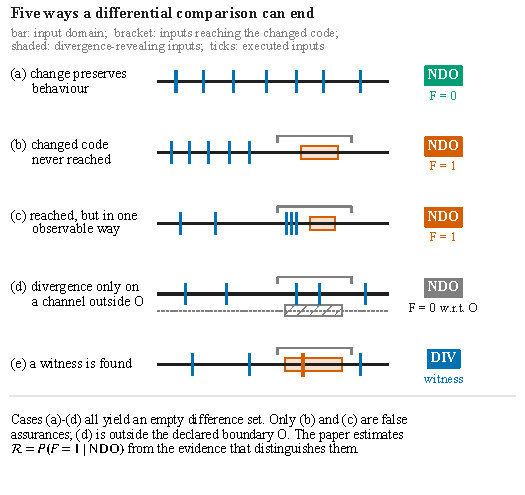
\includegraphics[width=\columnwidth]{figures/fig_motivation.pdf}
\caption{Five ways a differential comparison can end. Cases (a)--(d) all produce an empty difference set and the same \NDO{} verdict, but only (a) is correct; (b) and (c) are false assurances, and (d) lies outside the declared observation boundary $\obs$. The figure is conceptual.}
\label{fig:motivation}
\end{figure}

\paragraph*{Problem} This paper studies how reliable that reassurance is. We call the verdict issued when a comparison observes no divergence \NDOfull{} (\NDO{}) and ask how often it is wrong. We do not ask whether the versions are equivalent; that question is undecidable in general and belongs to regression verification~\cite{godlin2009regression,lahiri2012symdiff}. Our question is narrower and empirical. Given the evidence behind a particular \NDO{} verdict, how likely is it that an independent examination of the same change, within a declared observation boundary and adjudication budget, would find a divergence? We call this probability the \emph{false-assurance risk} of the verdict.

\paragraph*{What trusting the verdict requires} An \NDO{} verdict is the conjunction of several distinct claims, and each can fail independently:
\begin{enumerate}
\item \emph{observation}: no input in the executed set produced a difference on the compared channels;
\item \emph{sufficiency}: those inputs reached the changed code in enough observably distinct ways for a difference to have shown;
\item \emph{integrity}: the recorded evidence is what was actually observed, and the program under test did not alter it;
\item \emph{provenance}: the inputs were not derived from the labels or the expected answer;
\item \emph{responsiveness}: whatever turns the evidence into a judgment reacts correctly when the evidence weakens, strengthens or is tampered with;
\item \emph{equivalence}: the versions agree on all inputs and channels.
\end{enumerate}
Testing establishes only claim~1. Equivalence (claim~6) is out of reach of any finite observation (Remark~\ref{rem:equiv}). This paper is about claims 2--5: whether they can be made explicit, estimated, enforced and tested, and how much they change the probability that claim~1 misleads.

\paragraph*{Gap} Adjacent work bears on the question without answering it (Section~\ref{sec:background}):
\begin{itemize}
\item Coverage, mutation and checked-coverage analyses assess how strong a passing \emph{test suite} is for one program version~\cite{inozemtseva2014coverage,jia2011analysis,schuler2011assessing}. They do not attach an error probability to a no-divergence verdict on a version pair.
\item Selective prediction supplies the right estimand, risk among accepted predictions at a given coverage~\cite{elyaniv2010foundations,geifman2017selective}, and conformal methods supply guarantees under exchangeability~\cite{angelopoulos2024conformal}. Neither defines what the evidence behind a software verdict is, nor how an estimate should react when that evidence is degraded or tampered with.
\item The closest recent work measures the dataset-level accuracy of an ``all tests agree'' label~\cite{ayub2026semadiff}. It neither conditions on per-verdict evidence nor abstains.
\end{itemize}

\paragraph*{Approach} We treat an \NDO{} verdict as a selective prediction whose reliability is estimated from a structured description of its evidence. This reformulation yields three formal results (Section~\ref{sec:problem}). Risk measured under a declared boundary and budget is a lower bound for any wider boundary or stronger budget (Proposition~\ref{prop:mono}). An adversary who can write evidence can force any verdict issued on unvalidated evidence, so integrity must gate every verdict, including witnessed divergences (Proposition~\ref{prop:integrity}). And whether an estimator responds correctly to its evidence is logically independent of how accurate it is, so the two must be tested separately (Proposition~\ref{prop:indep}). We implement the formulation in \sbg{}, the eighth iteration of the Software Behavior Genome research prototype, which consists of four components:
\begin{enumerate}
\item a formal estimand $\R=P(F{=}1\mid\NDO{})$ relative to an observation boundary, an adjudication budget and a population;
\item a change-conditioned evidence profile and a calibrated, abstaining decision procedure (change-conditioned evidence calibration, \cec{});
\item an Evidence Response Signature (\ers{}) of eight properties, tested by controlled perturbations of the evidence;
\item an evidence-collection pipeline whose integrity is a precondition of every verdict.
\end{enumerate}

\paragraph*{Findings} We evaluate \sbg{} in a pilot on 312 executed development pairs from 101 synthetic programs, 31 QuixBugs programs and 43 BugsInPy bugs in 12 projects; 258 pairs have construction labels. The results are mixed, and we report them as they are.
\begin{itemize}
\item Plain differential testing had an observed false-assurance risk of 0.169 (31 of 183 \NDO{} verdicts).
\item The predecessor's sufficiency gate abstained on two thirds of those verdicts without lowering the rate (0.213).
\item As a label-free conformance test, \ers{} found a real defect in the evidence profile, corroborated it under real execution, and showed that the predecessor's verdicts ignore integrity failures.
\item As a source of predictive features, the richer evidence was \emph{not} shown to help. At matched coverage, full \cec{} differed from coverage-only calibration by 1.6 percentage points, with an interval from $-6.6$ to $+16.3$ and a sign that changes across seeds. Only differences of about 16 points were detectable.
\item The project's own ``five-dataset'' artifact turned out to be template-generated with label-derived outcomes, so this paper excludes it as evidence.
\end{itemize}

Table~\ref{tab:contrib} maps the contributions to the research questions and to the evidence that supports each.

\begin{table*}[!t]
\caption{Contributions, research questions, evidence and status. Status uses three levels: supported, partly supported, and not demonstrated.}
\label{tab:contrib}
\centering
\scriptsize
\setlength{\tabcolsep}{3pt}
\begin{tabular}{|c|L{4.2cm}|c|L{4.6cm}|L{4.0cm}|}
\hline
Id & Contribution & RQ & Evidence & Status \\
\hline
C1 & False-assurance estimand for \NDO{} verdicts, separated from equivalence; four propositions on abstention, boundary monotonicity, integrity and conformance (Section~\ref{sec:problem}) & -- & Definitions; Propositions~\ref{prop:integrity}--\ref{prop:indep} with proofs & Formal contribution \\
C2 & Change-conditioned evidence profile and \cec{} decision procedure with an integrity-first trust gate (Section~\ref{sec:approach}) & RQ3, RQ4 & 258 labelled pairs; matched-coverage contrasts & Implemented; predictive advantage not demonstrated \\
C3 & \ers{}: eight properties, ten perturbations, pass criteria with N/A and abstention accounting (Section~\ref{sec:ers}) & RQ2 & 312 records $\times$ 6 predictors; 30-pair real-execution analogue & Supported as a conformance test; not supported as predictive features \\
C4 & Trusted evidence collection with a bounded threat model (Section~\ref{sec:trust}) & RQ1 & macOS re-run (25), Linux probes (125) & Partly supported: fail-safe for keyless writers; detection only for in-process forgery; one open channel \\
C5 & Matched-coverage evaluation protocol with power analysis (Section~\ref{sec:design}) & RQ3, RQ4 & Bootstrap, Holm, MDE & Supported; result inconclusive (underpowered) \\
C6 & Evidence audit and traceability: claim register, exclusion of a label-derived artifact, cross-platform status (Sections~\ref{sec:res-rq5}, \ref{sec:repro}) & RQ5 & Static audit; register; saved outputs & Supported \\
\hline
\end{tabular}
\end{table*}

\paragraph*{Non-claims} The paper does not claim:
\begin{itemize}
\item that \NDO{} establishes equivalence;
\item that \sbg{} detects every divergence;
\item that post-hoc perturbations estimate causal effects;
\item that \ers{} features improve prediction;
\item that the collector is secure against arbitrary programs;
\item that any result generalises beyond the development corpus.
\end{itemize}
Independent human adjudication has been designed and implemented but not carried out. External benchmark subjects (QuixBugs, BugsInPy) were executed only as development data, and no benchmark was held out.

\paragraph*{Organisation} Section~\ref{sec:background} reviews related work. Section~\ref{sec:problem} formalises the system model. Sections~\ref{sec:approach}--\ref{sec:trust} present the methodology, \ers{} and the trust architecture. Section~\ref{sec:design} gives the evaluation design and Section~\ref{sec:results} the results by research question. Sections~\ref{sec:discussion}--\ref{sec:repro} cover discussion, threats to validity and reproducibility.
